\chapter{Klasy}

W systemie będą istnieć trzy podstawowe klasy (rys 5.1). Pierwszą z nich będzie \texttt{object}, będąca klasą bazową dla klas opisujących postacie, zwierzęcia, rośliny i terenu. Służyć będzie do opisu obiektu w przestrzeni. 
Drugą klasą podstawową będzie \texttt{state}, będąca klasą bazową dla dziedziczących klas opisujących stan postaci (\texttt{character\_state}) i stan zwierzęcia (\texttt{animal\_state}). Klasy te opisywać będą stan odpowiednich obiektów. Odziedziczą po nich klasy odpowiadające stanom postaci i zwierząt z diagramów stanów (np. \texttt{character\_passive \_state}).
Trzecią klasą podstawową będzie \texttt{material}. Opisywać będzie jakie surowce można zebrać i jakie surowce gracz będzie mieć w ekwipunku. Obiekty tej klasy zawierać się będą w listach obiektów roślin, zwierząt i będą częścią ekwipunku gracza.
Klasa postaci opisze postać gracza, jej parametry (życie, najedzenie, temperaturę), ekwipunek i stan.
Klasa \texttt{animal} opisze obiekt zwierzęcia, jego życie, stan i dostępne do zebrania z niego surowce.
Klasa \texttt{plant} opisze jakie surowce są dostępne do zebrania z danej rośliny.
Klasa \texttt{terrain} opisze ukształtowanie terenu.

\begin{figure}[H]
    \centering
        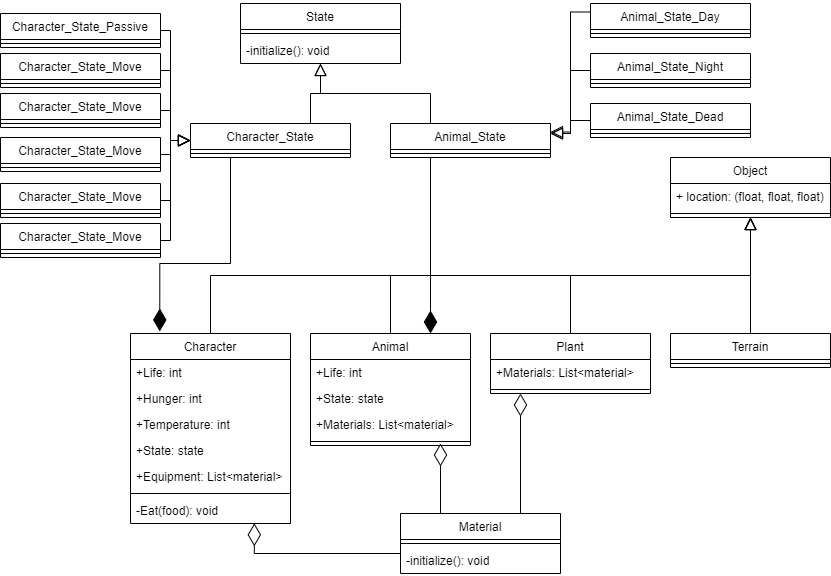
\includegraphics[width=0.97\textwidth]{Graphics/classes.png}
         \index{Diagram klas}
         \caption{Diagram klas}
\end{figure}

%Trzeba opisać wykorzystane algorytmy